% chktex-file 18 
% chktex-file 46 

\documentclass{isprs} % isprs class modified 23-04-2019 (Dennis Wittich)
\usepackage{subfigure}
\usepackage{setspace}
\usepackage{geometry} % added 27-02-2014 Markus Englich
\usepackage{epstopdf}
\usepackage[labelsep=period]{caption}  % added 14-04-2016 Markus Englich - Recommendation by Sebastian Brocks
\usepackage[british]{babel} 
\usepackage[hang]{footmisc}
\def\footnotemargin{1em} % added 08-01-2020 Dennis Wittich

% //-- HL:
\usepackage{booktabs}
% \usepackage{flushend}
\usepackage{siunitx}
\usepackage{threeparttable}
\usepackage{url}
\newcommand{\ie}{ie}
\newcommand{\eg}{eg}
\usepackage{listings}
\usepackage{color}
\definecolor{codegreen}{rgb}{0,0.6,0}
\definecolor{codegray}{rgb}{0.5,0.5,0.5}
\definecolor{codepurple}{rgb}{0.58,0,0.82}
\definecolor{backcolour}{rgb}{0.95,0.95,0.92}
\lstdefinestyle{mystyle}{
    backgroundcolor=\color{backcolour},   
    commentstyle=\color{codegreen},
    keywordstyle=\color{magenta},
    numberstyle=\tiny\color{codegray},
    stringstyle=\color{codepurple},
    basicstyle=\footnotesize,
    breakatwhitespace=false,         
    breaklines=true,                 
    captionpos=b,                    
    keepspaces=true,                 
    numbers=left,                    
    numbersep=5pt,                  
    showspaces=false,                
    showstringspaces=false,
    showtabs=false,                  
    tabsize=2
}
\lstset{style=mystyle,basicstyle=\ttfamily\footnotesize,breaklines=true}
% --//

\usepackage[authoryear]{natbib}
\def\bibhang{0pt}

\geometry{a4paper, top=25mm, left=20mm, right=20mm, bottom=25mm, headsep=10mm, footskip=12mm} % added 27-02-2014 Markus Englich
%\usepackage{enumitem}

%\usepackage{isprs}
%\usepackage[perpage,para,symbol*]{footmisc}

%\renewcommand*{\thefootnote}{\fnsymbol{footnote}}
\captionsetup{justification=centering,font=normal} % thanks to Niclas Borlin 05-05-2016
\captionsetup[figure]{font=small} % added 23-04-2019 Dennis Wittich
\captionsetup[table]{font=small} % added 23-04-2019 Dennis Wittich

\begin{document}

% TODO: the title is perhaps too short? Or is good since it's punchy?
\title{Streaming CityJSON datasets}
% \title{CityJSONSeq: streaming massive CityJSON datasets}
% \title{Streaming massive CityJSON datasets with CityJSONSeq}


% KAO: Remove extra spacing
\author{
 Hugo Ledoux\textsuperscript{1}, Gina Stavropoulou\textsuperscript{1}, Balázs Dukai\textsuperscript{2}}

% KAO: Remove extra newline
\address{
	\textsuperscript{1 }Delft University of Technology, the Netherlands---\texttt{[h.ledoux, g.stavropoulou]@tudelft.nl}\\
	\textsuperscript{2 }3DGI, the Netherlands---\texttt{balazs.dukai@3dgi.nl}\\
}

% If the corresponding author is NOT the final author, always add a % space before the subsequent comma, i.e.
% first author name\textsuperscript{a,}\thanks{Corresponding author} , % second author name \textsuperscript{b}, etc.
% thanks to Niclas Borlin 05-05-2016
% information on the corresponding author should not be used any longer and has been commented out
% C. Heipke, Jan 03,2024

% the use of the information of commissions and working groups should not be used any longer and has been commented out
% C. Heipke, Sept. 20,2022
%\commission{XX, }{YY} %This field is optional. If filled, XX and YY should be replaced by adequate numbers. See https://www2.isprs.org/commissions/
%\workinggroup{XX/YY} %This field is optional.
%\icwg{}   %This field is optional.

\abstract{
% The abstract must have the following structure: 
% \begin{enumerate}
% \setlength\itemsep{0em}\setlength\parskip{0em}\setlength\topsep{0em}\setlength\partopsep{0em}\setlength\parsep{0em} 
% \item{Title of the contribution} 
% \item{Author(s) and affiliation}
% \item{Keywords (max. 6)}
% \item{Main body (one page max)}
% \item{Illustrations (one page max, optional)}
% \item{References (8 max, optional)}
% \end{enumerate}
% Abstracts must contain the title, the author(s) names incl. affiliations, the keywords and a summary of the contribution (research question, relevance, solution, evaluation).

We present \emph{CityJSON Text Sequences} (CityJSONSeq), a format based on \emph{JSON Text Sequences} and CityJSON\@. 
CityJSONSeq was added to the CityJSON version 2.0 standard that was recently released, and it allows us to stream very large 3D city models.
The main idea is to decompose a CityJSON dataset into its individual features (eg each Building, each Bridge, etc.) and create several indepedent JSON objects of a newly defined type: \texttt{CityJSONFeature}.
We elaborate on the engineering decisions that were taken to develop CityJSONSeq, we present the open-source software we have developed to convert to and from CityJSONSeq, and we discuss different aspects of the new format, \eg\ size, usability, etc.
We consider CityJSONSeq to be a better format than CityJSON because: (1) once serialised it is about 10\% more compact; (2) it takes an order of magnitude less time to process; and (3) it uses significantly less memory for certain operations.
}

\keywords{3D city modelling, CityJSON, CityGML, streaming}
\maketitle
%\saythanks % added 28-02-2014 Markus Englich


\sloppy


%%%
%
\section{Introduction}%
\label{sec:intro}
 
CityJSON is a JSON-based encoding for storing 3D city models that implements a subset of the latest version, v3.0.0, of the CityGML data model~\citep{OGC-CityGML3}.
As further described in \citet{19_ogdss_cityjson}, its development started in 2017 with the aim of offering an easy-to-use and web-ready alternative to the GML-encoded CityGML files~\citep{OGC-CityGML3-XML}, which in practice can be rather verbose, difficult to parse, and complex to manipulate.
The first official release of CityJSON (version 1.0) was a success: 
\begin{enumerate}
  \item its JSON-based files were on average around 7X more compact than their CityGML-GML equivalents without loss of information. See \citet{19_ogdss_cityjson} and \url{https://www.cityjson.org/filesize/}, and also \citet{Praschl23} for a comparison with standard computer graphics formats; 
  \item it was adopted as an OGC Community Standard~\citep{OGC-CityJSON-v10}; 
  \item it was adopted by the Dutch government as a 3D standard to distribute nation-wide 3D datasets; 
  \item several implementations and plugins have been developed, most notably FME\@.
\end{enumerate}



%

However, the version 1.0 of CityJSON had one limitation: its structure for storing the coordinates of the geometries (see Figure~\ref{fig:cj_idea}) made the \emph{streaming} of very large datasets complex, if not impossible.
Since city datasets are progressively becoming larger (it is not uncommon to have CityGML-GML files of over 2GB), the large data volume can hinder the processing of CityJSON files.
As further defined in Section~\ref{sec:streaming}, streaming refers to the possibility of downloading/transferring/processing a dataset without having to load it all in memory.

%

We present in this paper \emph{CityJSON Text Sequences} (\emph{CityJSONSeq} in short in the following), a format based on \emph{JSON Text Sequences}~\citep{IETF-JSONSeq} and CityJSON, and inspired by \emph{GeoJSON Text Sequences}~\citep{IETF-GeoJSONSeq}. 
CityJSONSeq was added to the CityJSON version 2.0 standard that was released in 2023 (and also standardised by the OGC, see \citet{OGC-CityJSON-v20}).
As further described in Section~\ref{sec:cityjsonseq}, the idea is to decompose a (often large) CityJSON file into its individual \emph{features} (\eg\ each \texttt{Building}, each \texttt{Bridge}, etc.) and create several JSON objects of a newly defined type \emph{CityJSONFeature}.
These objects are either serialised into a text file, or streamed from a server to client or from one application to another.
This allows us to avoid a long list of vertices that need to be indexed, as it is the case with CityJSON files (see Section~\ref{sec:cityjson} for details).
\begin{figure}
  \centering
  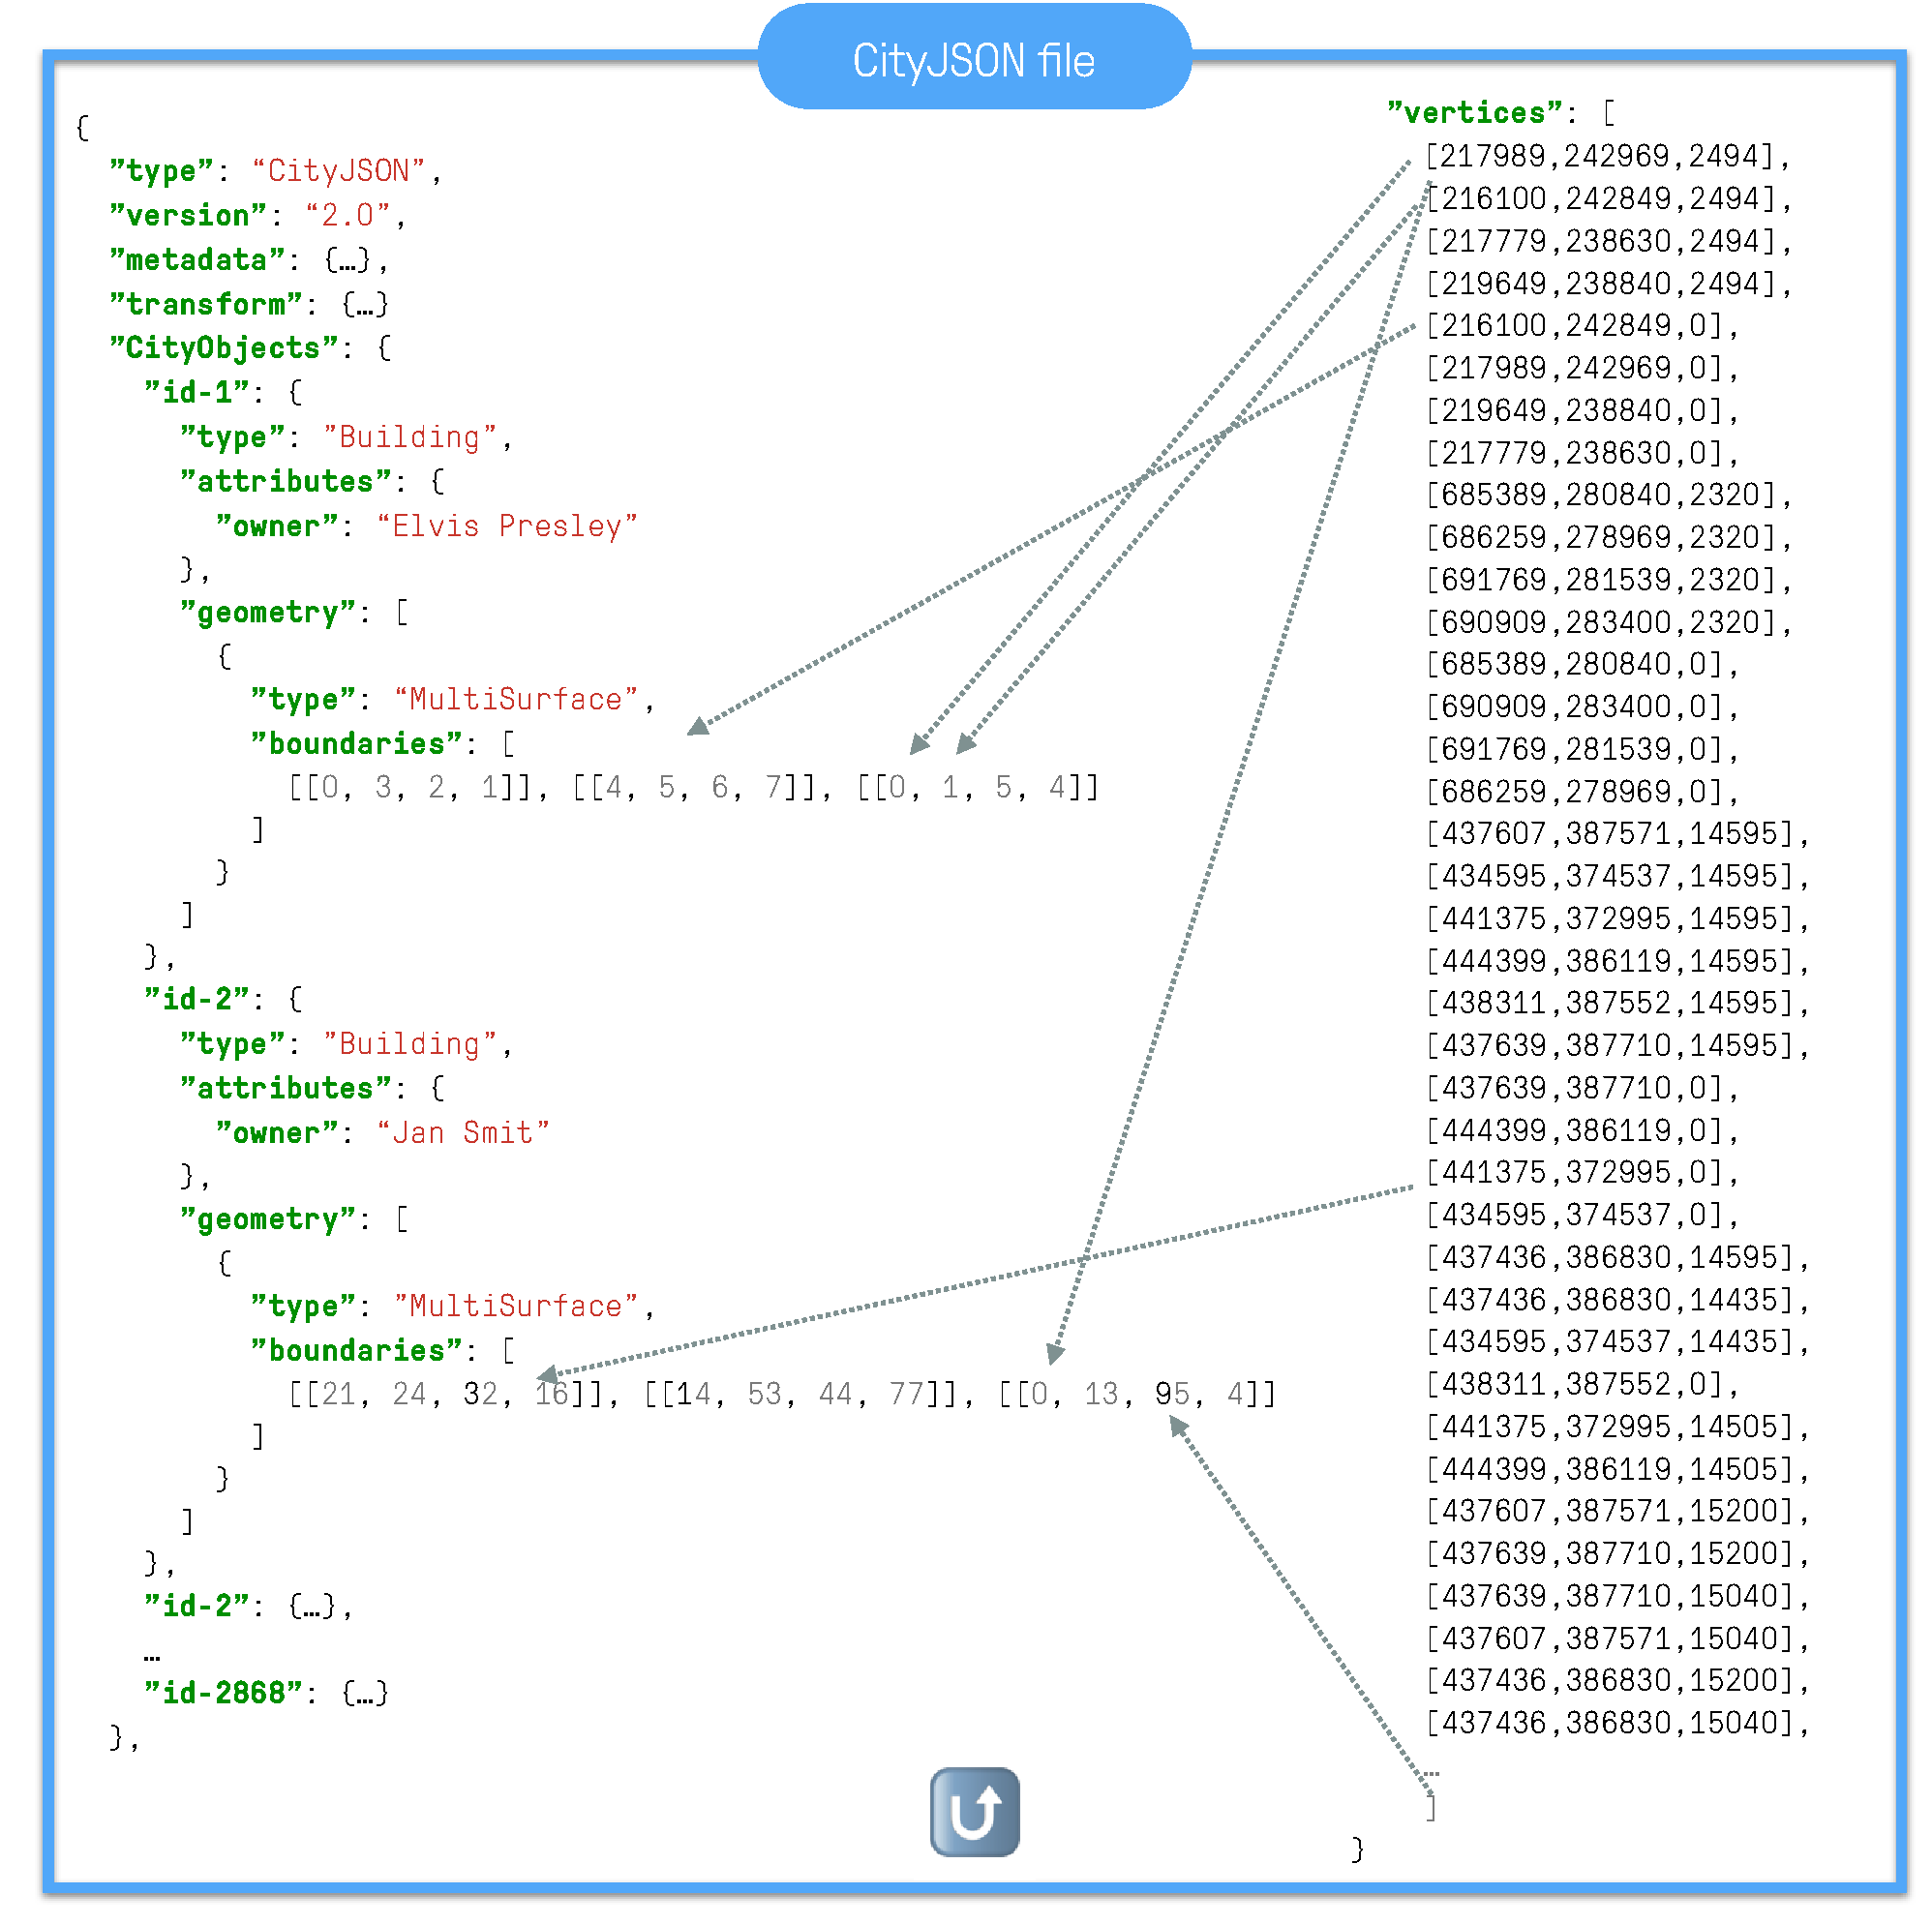
\includegraphics[width=0.95\linewidth]{figs/cj_idea}
  \caption{An example of a CityJSON file. The vertices are stored in a global list, and the position of the vertices in that list are used in the geometries (represented by the arrows, many have been left out for clarity).}%
\label{fig:cj_idea}
\end{figure}

%

We have implemented and released an open-source software to convert between CityJSON and CityJSONSeq objects; we describe it in Section~\ref{sec:experiments}.
We also analyse the size of CityJSONSeq files versus CityJSON files, and that for several real-world datasets.
It can be observed that one advantage of CityJSONSeq, besides that files containing thousands of features can be processed with a low memory footprint, is that it compresses further the CityJSON files by around 12\%, sometimes more.
We discuss in Section~\ref{sec:experiments} the reasons for this interesting finding.
Finally, we will also present the open-source software for processing streams of CityJSON datasets, that is currently being developed.

%%%
%
\section{Structure of a CityJSON file}%
\label{sec:cityjson}

% \begin{itemize}
%   \item global indexing of vertices make streaming impossible
%   \item discuss the geometry templates and other metadata
% \end{itemize}




As shown in Figure~\ref{fig:cj_idea}, a CityJSON object, which is a JSON object, represents a given geographical area, and it typically contains the following JSON properties: 
\begin{enumerate}
  \item \texttt{"type"}: it must be \texttt{"CityJSON"};
  \item \texttt{"version"}: \texttt{"2.0"} is the current version;
  \item \texttt{"metadata"}: different metadata related to the dataset can be stored. The most important is the definition of the coordinate reference system (CRS)
  \item \texttt{"transform"}: CityJSON \texttt{"vertices"} are compressed and stored as integers only. The parameters of this property allow us to convert from those integers back to real-world coordinates.
  \item \texttt{"CityObjects"}: a dictionary where the properties are the identifiers of the city objects (\emph{IDs}), which are any CityGML city object (for instance a \texttt{Building}, a \texttt{BuildingPart}, a \texttt{SolitaryVegetationObject}, etc.).
  Each of the city objects is listed one after the other, even if some are \texttt{"children"} of others.
  As an example, for a \texttt{Building} containing 2 parts, the 3 objects will be represented at the same level and linked by their \emph{IDs}, as shown in Figure~\ref{fig:parents_children}.
  The schema is thus flat and all hierarchies have been removed.
  Each city object can have a \texttt{"parents"} and/or a \texttt{"children"} property, and this is how in the snippet the building \texttt{"id-1"} is linked to its 2 parts.
  % We define 2nd-level city objects as having a \texttt{"parent"}.
  The fact that a dictionary is used means that developers have direct access to the city objects through their IDs (and also in constant time if a hashmap is used to implement the dictionary while parsing the file).
  \item \texttt{"vertices"}: The 3D geometric primitives are those of CityGML, and multi/composite solids with several parts are supported.
  A geometric primitive does not list all the coordinates of its vertices, rather the coordinates of the vertices are stored in a separate array (the \texttt{"vertices"} property of the CityJSON object), and the geometric primitives refer to the position of a vertex in that array.
  The indexing mechanism of the format \emph{Wavefront OBJ}\footnote{\url{https://en.wikipedia.org/wiki/Wavefront_.obj_file}} is reused, because it has been successfully used for many years in the computer graphics community.
  There are several advantages to this approach.
  First, the files can be compressed: 3D vertices are often shared by several surfaces, and repeating them can be costly, especially if they are very precise (sub-millimetre precision is often used).
  Second, this approach increases the topological relationships that are explicitly stored in the file, and several operations (\eg\ are 2 buildings adjacent?) can be sped up and made more robust.
  Third, it is very easy to convert to a representation listing all coordinates; the inverse is not true. 
  However, this is where the streaming of geometries is problematic: the array of "vertices" contains several millions vertices, especially for very large areas, .
  To be able to reconstruct one Building, all the \texttt{"vertices"} need to be in memory, which means waiting for millions of unused vertices to be loaded.
  \item \texttt{"appearances"}: Both textures and materials for surfaces are supported.  
  The material of a surface is represented with the X3D specifications\footnote{\url{https://en.wikipedia.org/wiki/X3D}}, and for the textures the COLLADA specifications\footnote{\url{https://www.khronos.org/collada/}} are reused.
  \item \texttt{"geometry-templates"} 
  Geometry templates are used to represent identical geometries several times, they only need to be defined once (and translations/rotations/scaling are applied).
  They are used for city objects like trees and lamp posts. 
\end{enumerate}


\begin{figure}
  \centering
\begin{lstlisting}
  "CityObjects": {
    "id-1": {
      "type": "Building",
      "attributes": {...},
      "children": ["id-2", "id-3"],
      "geometry": [{...}]
    },
    "id-2": {
      "type": "BuildingPart",
      "parents": ["id-1"],
      "geometry": [{...}]
      ...
    },
    "id-3": {
      "type": "BuildingPart",
      "parents": ["id-1"],
      "geometry": [{...}]
      ...
    }
    ...
    "id-77": {}
  }
\end{lstlisting}
  \caption{CityJSON mechanism to flatten out the schema: the city objects are stored in a flat list, and they are linked together with the properties \texttt{"parents"} and \texttt{"children"}.}%
\label{fig:parents_children}
\end{figure}




%%%
%
\section{Streaming (3D) datasets}%
\label{sec:streaming}

In the context of geo-information, a \emph{stream} is a sequence of data that is available over a period of time, and ``can be thought of as items on a conveyor belt being processed one at a time rather than in large batches''\footnote{From \url{https://en.wikipedia.org/wiki/Stream_(computing)}}.

%

For GML-based formats (which are feature-centric), modifying a file for the purpose of streaming is usually a simple task that involves sending the features in the dataset one-by-one.
However, notice that this is only true for simple files and GML features stored following the Simple Feature paradigm~\citep{OGC-SF}.
For more complex data models like CityGML where \emph{Implicit Geometries} and \emph{XLinks} are used, the conversion often needs a large amount of pre-processing.
\emph{XLinks} are links between elements in a file (similar to \emph{pointers} in a computer program), a concrete example in a CityGML file is a cube that lists the geometries of 5 of its surfaces, but its 6th surface is simply a link to another surface somewhere else in the file (which belongs to another building, for instance).
If in the stream the linked surface has not appeared yet, the receiver cannot process the cube and needs to wait for that specific 6th surface to appear.
It is not always possible to (re-)order a CityGML file so that all the references can be resolved without having to store locally information until it appears in the stream.
However, it is always possible to resolve the \emph{XLinks} before streaming a dataset (that is copy the geometry of the 6th surface to the cube), but this means that its size is increased, and that converting back to the original file will not be possible.

%

For the \emph{GeoJSON} format~\citep{IETF-GeoJSON}, which follows the Simple Feature paradigm, creating a stream is trivial since each of the features in the dataset becomes one JSON object and one line~\citep{IETF-GeoJSONSeq}.
There are no links possible between features, they are all independent.

%

For formats that use a global indexing of vertices (as mentioned above, CityJSON is one of them, and  most formats used in computer graphics for meshes also, \eg\ OBJ and STL), the reorganisation of the elements in a file is more complex but nonetheless possible.
\citet{Isenburg03} describe algorithms and tools that interleave the vertices and faces in a file (instead of having one large list of vertices at the end) and add simple tags to inform that vertices are not to be used anymore (and thus can be freed from memory).
This allows us, in theory, to process/edit/manipulate infinitely large meshes, since they never have to be completely loaded in memory.
The idea is exemplified by the construction of gridded terrains that are gigabytes in size~\citep{Isenburg06-1}.

However, this cannot be implemented in CityJSON directly as all the vertices need to be in the one JSON property \texttt{"vertices"}.


%%%
%
\section{CityJSON Text Sequences}%
\label{sec:cityjsonseq}

\begin{figure*}[h]
  \centering
  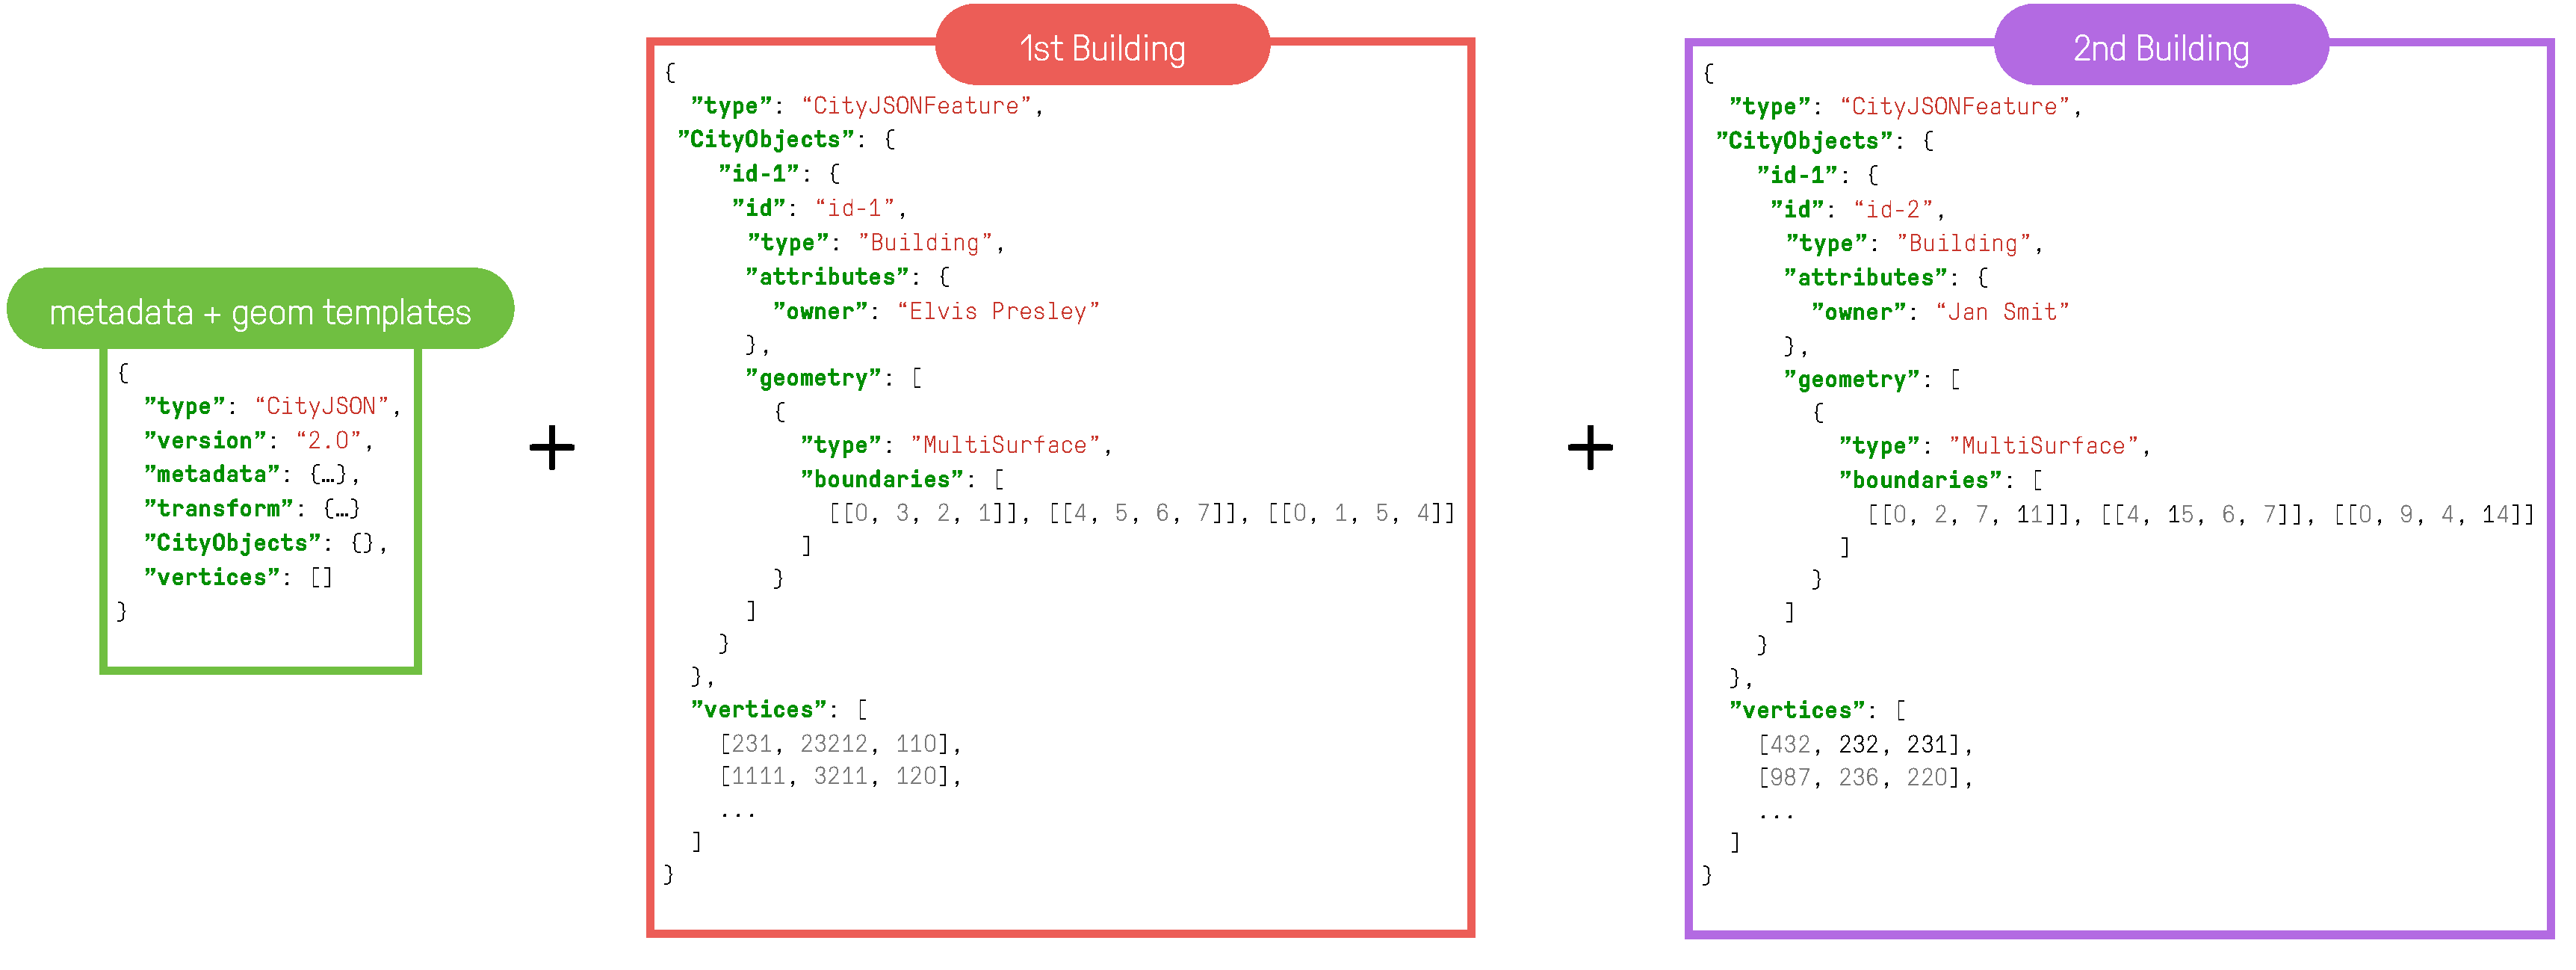
\includegraphics[width=0.95\linewidth]{figs/cjseq_idea}
  \caption{The CityJSONSeq of a CityJSON dataset with two buildings contains three JSON objects: one for the metadata, plus one for each building.}%
\label{fig:cjseq_idea}
\end{figure*}

As shown in Figure~\ref{fig:cjseq_idea}, a CityJSONSeq decomposes a CityJSON object into its \emph{City Objects} (or ``features'', for instance each building, each bridge, each road, etc.), to create a sequence of several JSON objects.
Those JSON objects are of a new type that was introduced in CityJSON v2.0: \texttt{CityJSONFeature}.
It allows the storage of a single feature, for instance a \texttt{Building} together with its ``children'' objects (\eg\ a \texttt{BuildingPart} and/or a \texttt{BuildingInstallation}). 
Unlike a CityJSON Object, each feature is independent. 
It has its own list of vertices (which is thus \emph{local} to be JSON object, and is usually rather small, see next section for details) and its own textures and materials (if any).
The allowed properties are shown below; notice that the \texttt{"id"} property is used to clearly identity the ``parent'' of the feature, in case there are many children.
\begin{lstlisting}
{
  "type": "CityJSONFeature",
  "id": "id-1", 
  "CityObjects": {
    "id-1": {
      "type": "Building", 
      "attributes": { 
        "roofType": "gabled roof"
      },
      "children": ["mybalcony"],
      "geometry": [...]
    },
    "mybalcony": {
      "type": "BuildingInstallation", 
      "parents": ["id-1"],
      "geometry": [...]
    }
  },
  "appearance": {...}
  "vertices": [...]
}
\end{lstlisting}

%

CityJSONSeq follows the specifications of \texttt{ndjson} (newline delimited JSON)\footnote{\url{https://github.com/ndjson/ndjson-spec/}} and two constraints are added for handling CityJSON\@:
\begin{enumerate}
  \item each JSON Object must conform to the \emph{JSON Data Interchange Format specifications}~\citep{IETF-JSON} and be written as a UTF-8 string;
  \item each JSON Object must be followed by a new-line (LF: \texttt{"\textbackslash n"}) character, and it may be preceded by a carriage-return (CR: \texttt{"\textbackslash r"});
  \item a JSON Object must not contain the new-line or carriage-return characters;
  \item the first JSON Object must be of type \texttt{CityJSON};
  \item the following JSON Objects are of type \texttt{CityJSONFeature}.
\end{enumerate}

Note that a \texttt{CityJSONFeature} object does not contain all the information that is required for parsing the feature. 
Most commonly, the \texttt{"transform"} property, the CRS, and the \texttt{"geometry-templates"} must be known by the client in order to correctly reconstruct and georeference the city objects. 
The rule \#4 ensures that those are available. 
The CityJSON object must contain \texttt{"transform"} and eventually the other properties if needed; \texttt{"CityObjects"} and \texttt{"vertices"} must be present but they must be empty (to ensure that the JSON object is valid).

%

The CityJSONSeq for Figure~\ref{fig:cjseq_idea} is shown in Figure~\ref{fig:stream}:
\begin{figure*}
  \begin{lstlisting}
  {"type":"CityJSON","version":"2.0","transform": {"scale":[1.0,1.0,1.0],"translate":[0.0, 0.0, 0.0]},"metadata":{"referenceSystem":"https://www.opengis.net/def/crs/EPSG/0/7415"},"CityObjects":{},"vertices":[]}
  {"type":"CityJSONFeature","id":"id-1","CityObjects":{...},"vertices":[...]} 
  {"type":"CityJSONFeature","id":"id-2","CityObjects":{...},"vertices":[...]} 
  \end{lstlisting}
\caption{An example of a CityJSONSeq stream containing 3 features.}%
\label{fig:stream}
\end{figure*}



%%%
%
\section{Experiments with real-world datasets}%
\label{sec:experiments}


To convert efficiently between CityJSON and CityJSONSeq files (and vice-versa), we have developed the open-source software \emph{cjseq}, freely available at \url{https://github.com/cityjson/cjseq/}.
The program takes care of not only the geometries, but also of the materials, textures, and geometry templates that the dataset could contain.
It contains two sub-commands: 
\begin{enumerate}
  \item \texttt{cat}: based on a CityJSON file, it outputs a CityJSONSeq;
  \item \texttt{collect}: it reads a CityJSONSeq from \emph{stdin}, collects the features, and outputs a CityJSON file (duplicates vertices are merged).
\end{enumerate}



%%%
\subsection{File size comparison}

\begin{table*}
  \centering
  \begin{threeparttable}
  \caption{The datasets used for the benchmark. }%
  \label{tab:datasets}
  \small
  \begin{tabular}
    {@{}lcccccrrrcrr@{}}\toprule
    &&  \multicolumn{3}{c}{\textbf{dataset}} && \multicolumn{3}{c}{\textbf{size of file}} && \multicolumn{2}{c}{\textbf{vertices}}   \\ 
    \cmidrule{3-5} \cmidrule{7-9} \cmidrule{11-12} 
     && CityObjects &  LoDs & appearance\footnotesize ${}^{\text{(a)}}$ && CityJSON & CityJSONSeq & compr.\footnotesize ${}^{\text{(b)}}$ && total & largest\footnotesize ${}^{\text{(c)}}$ \\
    \midrule
    \textbf{3DBAG}          && \qty{1110} bldgs & 0+1.2+1.3+2.2 & &&    \qty{6.7}{\mega\byte} & \qty{4.3}{\mega\byte} &  64\%  &&   \num{82509} &  \num{4112} \\
    \textbf{Helsinki}       && \qty{77231} bldgs   & 1+2   &         && \qty{600}{\mega\byte} & \qty{432}{\mega\byte} &  72\%  && \num{3038576} &  \num{2202} \\
    \textbf{Helsinki\_tex}  && \qty{77231} bldgs   & 1+2   & tex     && \qty{748}{\mega\byte} & \qty{675}{\mega\byte} &  90\%  && \num{3038576} &  \num{2202} \\
    \textbf{Ingolstadt}     && \qty{55} bldgs      & 3     &         && \qty{5.1}{\mega\byte} & \qty{4.0}{\mega\byte} &  78\%  &&   \num{87972} & \num{12800} \\
    \textbf{Montréal}       && \qty{294} bldgs     & 2     & tex     && \qty{5.4}{\mega\byte} & \qty{4.6}{\mega\byte} &  85\%  &&   \num{31585} &  \num{3393} \\
    \textbf{NYC}            && \qty{23777} bldgs   & 2     &         && \qty{105}{\mega\byte} &  \qty{95}{\mega\byte} &  90\%  && \num{1035804} &  \num{2608} \\
    \textbf{Railway}        && \qty{50} diff       & 3     & tex+mat && \qty{4.5}{\mega\byte} & \qty{4.2}{\mega\byte} &  93\%  &&   \num{73554} & \num{14966} \\
    \textbf{Rotterdam}      && \qty{853} bldgs     & 2     & tex     && \qty{2.6}{\mega\byte} & \qty{2.7}{\mega\byte} & 104\%  &&   \num{22246} &   \num{631} \\
    \textbf{Vienna}         && \qty{307} bldgs     & 2     &         && \qty{5.4}{\mega\byte} & \qty{4.8}{\mega\byte} &  89\%  &&   \num{47220} &  \num{2025} \\
    \textbf{Zürich}         && \qty{52834} bldgs   & 2     &         && \qty{279}{\mega\byte} & \qty{247}{\mega\byte} &  89\%  && \num{3472989} &  \num{4069} \\
    \bottomrule
  \end{tabular}
    \begin{tablenotes}[flushleft]
      \footnotesize
      \item ${}^{\text{(a)}}$ `tex' is textures stored; `mat' is material stored
      \item ${}^{\text{(b)}}$ compression is $\frac{CityJSONSeq}{CityJSON}$, smaller is better
      \item ${}^{\text{(c)}}$ number of vertices in the largest feature of the stream
    \end{tablenotes}
  \end{threeparttable}
\end{table*}

With \emph{cjseq}, we have converted several publicly available files (details of files at \url{https://github.com/cityjson/paper_cjseq/tree/main/data}), and Table~\ref{tab:stats} shows an overview of the files stored both in CityJSON and CityJSONSeq.
% TODO: setup website for hosting the files

First observe that---contrary to intuition---the size of a dataset serialised as a CityJSONSeq file is around 12\% more compact than serialised as a CityJSON file, and in the case of \textbf{3DBAG} it is 36\% compacter.
The main reason for this is that the indices of the vertices are low integers for each feature (because the lowest index in each feature is always ``0''), and do not increase to several millions.
For instance, the dataset \textbf{Helsinki} contains a total of more than 3 millions vertices, but its largest feature contains only but 2202 vertices.
The fact that many indices are used for representing the geometries (and for the textures) means that if several large numbers are used then the size of the file will grow; if they maximum vertex index is around 2000 for each feature, then the file size will be less than the original file.

%

Only one dataset sees its size slightly increased when serialised to a CityJSONSeq file (\textbf{Rotterdam}).
This is caused, primarily, by the fact that the dataset has textures that are shared by most of the buildings, and the \texttt{"appearance"} property must be repeated for each of the feature (in the CityJSON file it is only stored once and referenced by all buildings).
If we remove the textures from the CityJSON file it is \qty{2.1}{\mega\byte} and its CityJSONSeq equivalent is \qty{1.3}{\mega\byte} (which means a difference of 62\%)


%%%
\subsection{Processing speed comparison}

We compare the speed and memory footprint of accessing each city object in a dataset.
This operation is common in applications that manipulate city models.

When a city model is stored in its entirety in one CityJSON object, we need to load the whole CityJSON object into memory in order to access the \texttt{"transform"} and \texttt{"vertices"} properties for instance.

With a CityJSONSeq file, we can read the file line by line, processing and discarding the city objects one by one.
As shown in the experiments below, this allows for very efficient operations in terms of both CPU and memory usage.
Operations that would highly benefit from this are subsetting and merging a citymodel.
Operations like modifying the CRS or updating the metadata would not even require to loop through the features, just to alter the first object in the file.

%

We have processed all the datasets from Table~\ref{tab:datasets} with two simple Python scripts that loop through the city objects and their geometries, and increment a global counter for the geometry type (\texttt{Solid} or \texttt{MultiSurface}).
This is just an example of a simple local operation, any other operation such as calculating the area of the façades or counting the number of windows could have been performed.
The results for both the maximum memory footprint\footnote{The resident set size (RSS) was used, which is the portion of main memory occupied by the Python script.} and the time used are shown in Table~\ref{tab:ramtime}.
The scripts are available at \url{https://github.com/cityjson/paper_cjseq/tree/main/scripts/}.
\begin{table*}
  \centering
  \caption{Comparison of the processing time and max RAM use for processing the same data stored in a CityJSON file and a CityJSONSeq file.}
  \small
  \begin{tabular}
    {@{}lcrrcrrr@{}}\toprule
    &&  \multicolumn{2}{c}{\textbf{RAM used (MB)}} && \multicolumn{3}{c}{\textbf{time (s)}} \\ 
    \cmidrule{3-4} \cmidrule{6-8} 
     && CityJSON & CityJSONSeq && CityJSON & CityJSONSeq & diff \\
    \midrule
     \textbf{3DBAG}         &&   76.9 & 16.1  &&   0.10 & 0.07 & 1.4 \\
     \textbf{Helsinki}      && 3743.1 & 15.0  &&  13.39 & 2.74 & 4.9 \\
     \textbf{Helsinki\_tex} && 5004.8 & 19.1  &&  29.60 & 4.72 & 6.3 \\
     \textbf{Ingolstadt}    &&   65.5 & 21.3  &&   0.08 & 0.06 & 1.3 \\
     \textbf{Montréal}      &&   79.3 & 20.8  &&   0.11 & 0.07 & 1.6 \\
     \textbf{NYC}           &&  949.5 & 16.0  &&   1.78 & 0.70 & 2.5 \\
     \textbf{Railway}       &&   69.6 & 29.6  &&   0.09 & 0.07 & 1.3 \\
     \textbf{Rotterdam}     &&   42.4 & 14.6  &&   0.04 & 0.04 & 1.0 \\
     \textbf{Vienna}        &&   60.1 & 15.7  &&   0.06 & 0.05 & 1.2 \\
     \textbf{Zurich}        && 2793.1 & 16.3  &&   6.05 & 2.00 & 3.0 \\
    \bottomrule
  \end{tabular}%
  \label{tab:ramtime}
\end{table*}

The results indicate that there is a very significant benefit to using CityJSONSeq, compared to regular CityJSON files, at least for operations that do not require analysing or calculating city objects that are close to each other.
Operations like calculating volumes, merging and subsetting files, finding city objects with specific attributes, etc.\ will all use significantly less memory and will be significantly faster.


%%%
%
\section{Discussion and future work}%
\label{sec:discussion}

\begin{itemize}
  \item We have kept most of the structure of CityJSON so that parsers do not need to be adapted much.
  \item CityJSONSeq is an attractive alternative to CityJSON, in most uses it is better to use since it is compacter, processing it uses less memory and is faster.
  \item CityJSONSeq is an attractive alternative to CityJSON; in most uses it is more compact, its processing requires less memory and it is faster.
  \item We have kept most of the structure of CityJSON so that parsers do not need to be adapted much.
  \item it opens up many possibilities for processing large 3dcm by using Unix pipes. A few of the tools developed for CityJSON are already reading/writing to stdin/stdout, so they can be chained together.
  \item cjseqview, cjseqval are two of them, but developing others to eg filter, calculate volumes or repair geometries would be trivial
  \item the nice part is that the tools do not need to be written in the same language, one pipeline can have tools built in Python and Rust and C++ and it all works nicely.
  \item extensions: these should be placed in the metadata or collection
\end{itemize}

Disadvantages:
\begin{itemize}
  \item  Software implementing CityJSON need to account for both regular CityJSON and CityJSONSeq.
  \item  In case of many, small, interconnecting CityObjects, a global vertex list would provide better compression than the separate vertex lists of the CityJSONFeatures.
  \item  Appearances (esp. Material) are relatively heavy objects with many properties. If an appearance is shared across most CityObjects, duplicating it in each Feature could negate the effect of small vertex indices and actually increase the file size compared to a regular CityJSON file. This is just theorizing, haven't tested.
\end{itemize}

% TODO: add conclusions

{
	\begin{spacing}{1.17}
		\normalsize
		\bibliography{refs} % Include your own bibliography (*.bib), style is given in isprs.cls
	\end{spacing}
}

\end{document}
